\setcounter{chapter}{13}
\chapter{Radioactivité}

\section{Vocabulaire et rappels}
\subsection{Rappels}

\blocrouge{A savoir}{
	\begin{itemize}
		\item Le noyau d'un atome est formé de protons et de \trou{neutrons}.
		\item Un élément est défini par son numéro atomique Z (c'est le nombre \trou{de protons}) et son symbole chimique.	
		\item Le nombre de masse est noté: A . Il correspond aux nombres de \trou{nucléons} présents dans le noyau (nombre de \trou{protons} + \trou{nombre de neutrons}
		\item La notation symbolique d'un noyau  X est $$_Z^A X$$
		\item Deux noyaux possédant le même numéro atomique mais un nombre de masse différent sont appelés \trou{isotopes}.
	\end{itemize}

}

\etiquette{Application} On considère 3 noyaux: $_{40}^{93}Zr$ ; $_{238}^{92}U$ ; $_{40}^{95}Zr$. 
\begin{enumerate}
	\item Faire l'inventaire des particules contenues dans ces noyaux.
	\item Quels sont ceux qui sont isotopes ? Justifier.
\end{enumerate}

\vspace{4cm}

\subsection{Transformation nucléaire}

La physique nucléaire étudie les propriétés des noyaux des atomes. On observe que certains noyaux peuvent modifier leur composition. Ainsi le nombre de protons et de neutrons est modifié (selon certaines règles...). Ces modifications s'appellent des transformations nucléaires ou encore radioactivité.

\etiquette{Radioactivité alpha}

Une particule $\alpha$ est le nom donné au noyau d'hélium formé de\trou{ 2 protons et 2 neutrons}. 

Exemple de transformation: $$_{94}^{238}Pu \longrightarrow _{2}^{4}He + _{92}^{234}U$$

\blocrouge{Lois de conservation}{Toutes les transformations nucléaires valident 2 lois de conservation:
	\begin{enumerate}
		\item Conservation du nombre de charge 
		\item Conservation du nombre de masse
	\end{enumerate}

}

\etiquette{Radioactivité beta}
Il existe deux types de radioactivité bêta selon que la particule émise est chargée positivement ou négativement.
\begin{itemize}
	\item Radioactivité $\beta^-$ émission d'un électron: $_{-1}^{0}e$. Transformation d'un \trou{neutron} en proton. 
	\item Radioactivité $\beta^+$ émission d'un positron ou positon: $_{+1}^{0}e$. Transformation d'un \trou{proton en neutron}. 
\end{itemize}

\etiquette{Exemples}
\begin{itemize}
	\item Identifier le type de radioactivité
	\item Compléter les transformations chimiques
\end{itemize}

 $$^{238}_{92}U \longrightarrow ^{\trou{234}}_{90}Th + ^{4}_{\trou{2}}He$$

   $$^{11}_{6}C \longrightarrow ^{\trou{11}}_{\trou{5}}B + e^+
$$
  $$^{14}_{7}N \longrightarrow ^{14}_{6}C + \trou{e^- }$$
  
     \subsection{Diagramme (N,Z)}
     
    Sur un diagramme, on repère un noyau par son nombre de protons Z (en abscisse) et son nombre de neutron N (en ordonnée).
    
    Le diagramme complet: \url{https://segree.web-labosims.org/index.html}

    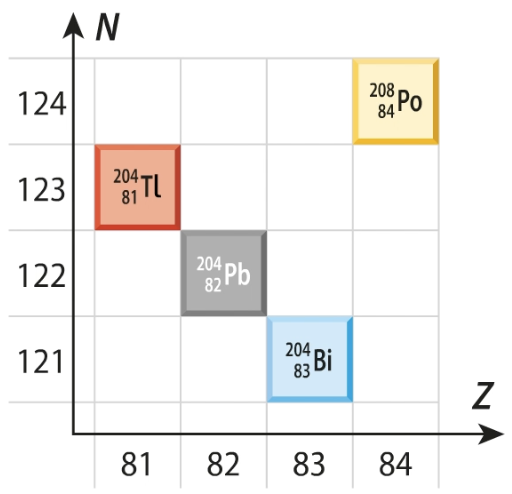
\includegraphics[width=.5\textwidth]{figures/diagramme_NZ}
    
    Les éléments qui ont la même abscisse sont \trou{isotopes}.
    \etiquette{Diagramme et radioactivité} Indiquer par une flèche sur le diagramme les transformations qui mènent les noyaux représentés au plomb.
    Pour chaque transformation, nommer le type de radioactivité.
    
    
\section{Evolution temporelle d'un échantillon radioactif}
\subsection{Cadre et objectif}
On modélise un échantillon de matière radioactive par une collection de noyaux radioactifs. On note $N(t)$ le nombre de ces noyaux. Au cours du temps, de manière \trou{aléatoire} chaque noyau va se désintégrer (et donner naissance à d'autres noyaux) ainsi $N(t)$ décroît au cours du temps. On veut connaître l'expression de  $N(t)$ en fonction de $t$. (voir TP)

\subsection{Activité d'un échantillon radioactif}

\blocrouge{Définition}{L'activité d'un échantillon est égale au nombre de noyaux qui se désintègrent \trou{par seconde}. Elle se note $A(t)$ et s'exprime en \trou{Becquerel} de symbole Bq.}

\etiquette{Démonstration} Preuve que $A(t)=-\frac{dN(t)}{dt}$
\begin{itemize}
	\item A t=0 s, on dispose d'un échantillon contenant $N_0$ noyaux radioactifs.
	\item A l'instant t>0, on veut estimer le nombre de noyaux qui se désintègrent par seconde: $A(t)$.
	\item On peut estimer $A(t)$ en raisonnant sur une durée $\Delta t$ alors: $$A(t)\approx \frac{N(t)-N(t+\Delta t)}{\Delta t}=-\frac{\trou{N(t+\Delta t)-N(t)}}{\Delta t}$$
	\item  Faisons tendre $\Delta t$ vers 0 pour estimer plus \trou{précisément} $A(t)$
	\item On reconnaît la limite d'un taux d'accroissement, on a donc $$A(t)=-\frac{dN(t)}{dt}$$
\end{itemize}

\subsection{Interprétation Graphique}
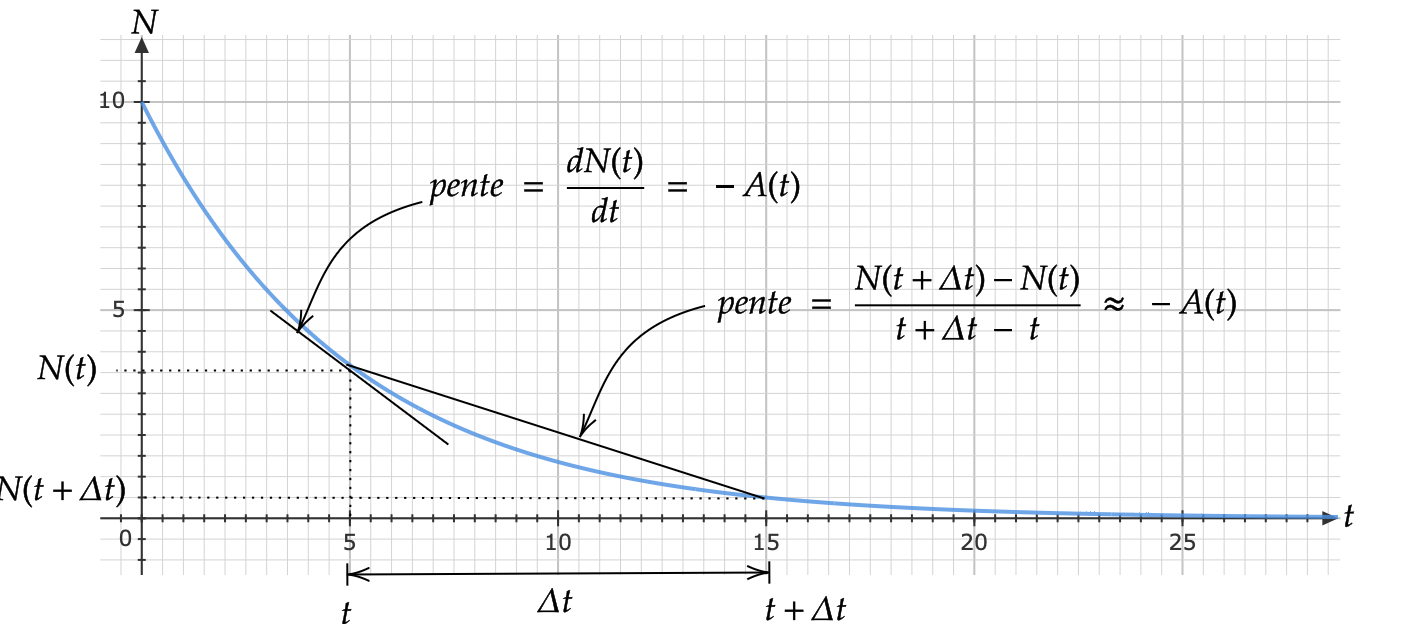
\includegraphics[width=.9\textwidth]{figures/decroissance}

L'activité à l'instant t s'obtient graphiquement en déterminant la \trou{pente} de la \trou{tangente} à la courbe N(t) à l'instant t. Analogue à la vitesse de disparition en chimie.

\subsection{Equation différentielle}

\etiquette{Propriété} On admet que l'activité $A(t)$ est \trou{proportionnelle} au nombre de noyaux radioactifs présents $N(t)$. Ce qui s'écrit $$A(t)=\lambda\times \trou{N(t)}$$


$\lambda$ est appelée la constante radioactive, sa valeur dépend du noyau considéré. Son unité est \trou{la seconde}.
\etiquette{Recherche de N(t)}

En utilisant la définition de $A(t)$ et la propriété ci-dessus on a $$\frac{dN(t)}{dt}=- \lambda \cdot N(t)$$

La solution générale s'écrit: $$N(t)=K\times e^{\trou{-\lambda t}}$$
Calcul de K à l'aide d'une condition initiale, on sait que $N(t=0\:s) = N_0$
$$N(0)=K\times e^0 = N_0 \Rightarrow K=\trou{N_0}$$
\blocrouge{A retenir}{ A tout instant $t\geqslant 0$, $$N(t)=\trou{N_0\times e^{-\lambda t}}$$}


On obtient $A(t)$ par dérivation $$A(t)= -\frac{dN(t)}{dt}=\lambda N_0 e^{-\lambda t}$$

\blocrouge{A retenir}{ A tout instant $t\geqslant 0$, $$A(t)=\trou{A_0\times e^{-\lambda t}}$$ avec $A_0=\lambda N_0$}

\subsection{Conséquences}
Le nombre de noyaux radioactifs et l'activité d'un échantillon décroissent exponentiellement. Le temps caractéristique de cette décroissance est appelé \trou{la demi-vie} (analogue au temps de demi-réaction en chimie)

\etiquette{Exercice} On dispose d'un échantillon contenant à t=0 $N_0$ noyaux radioactifs. Au bout de combien de temps, la moitié de ces noyaux se seront désintégrés.
\vspace{5cm}
\blocrouge{Définition}{La demi-vie est la durée au bout de laquelle la moitié des noyaux radioactifs d'un échantillon se sont désintégrés. Elle se note $t_{1/2}$ et s'exprime en seconde. On a la relation: $$t_{1/2}=\trou{\frac{\ln 2}{\lambda}}$$ }

\etiquette{Exercice} Représenter graphiquement l'allure de $N(t)$ et indiquer comment on détermine $t_{1/2}$

\newpage
\etiquetterouge{Résumé}

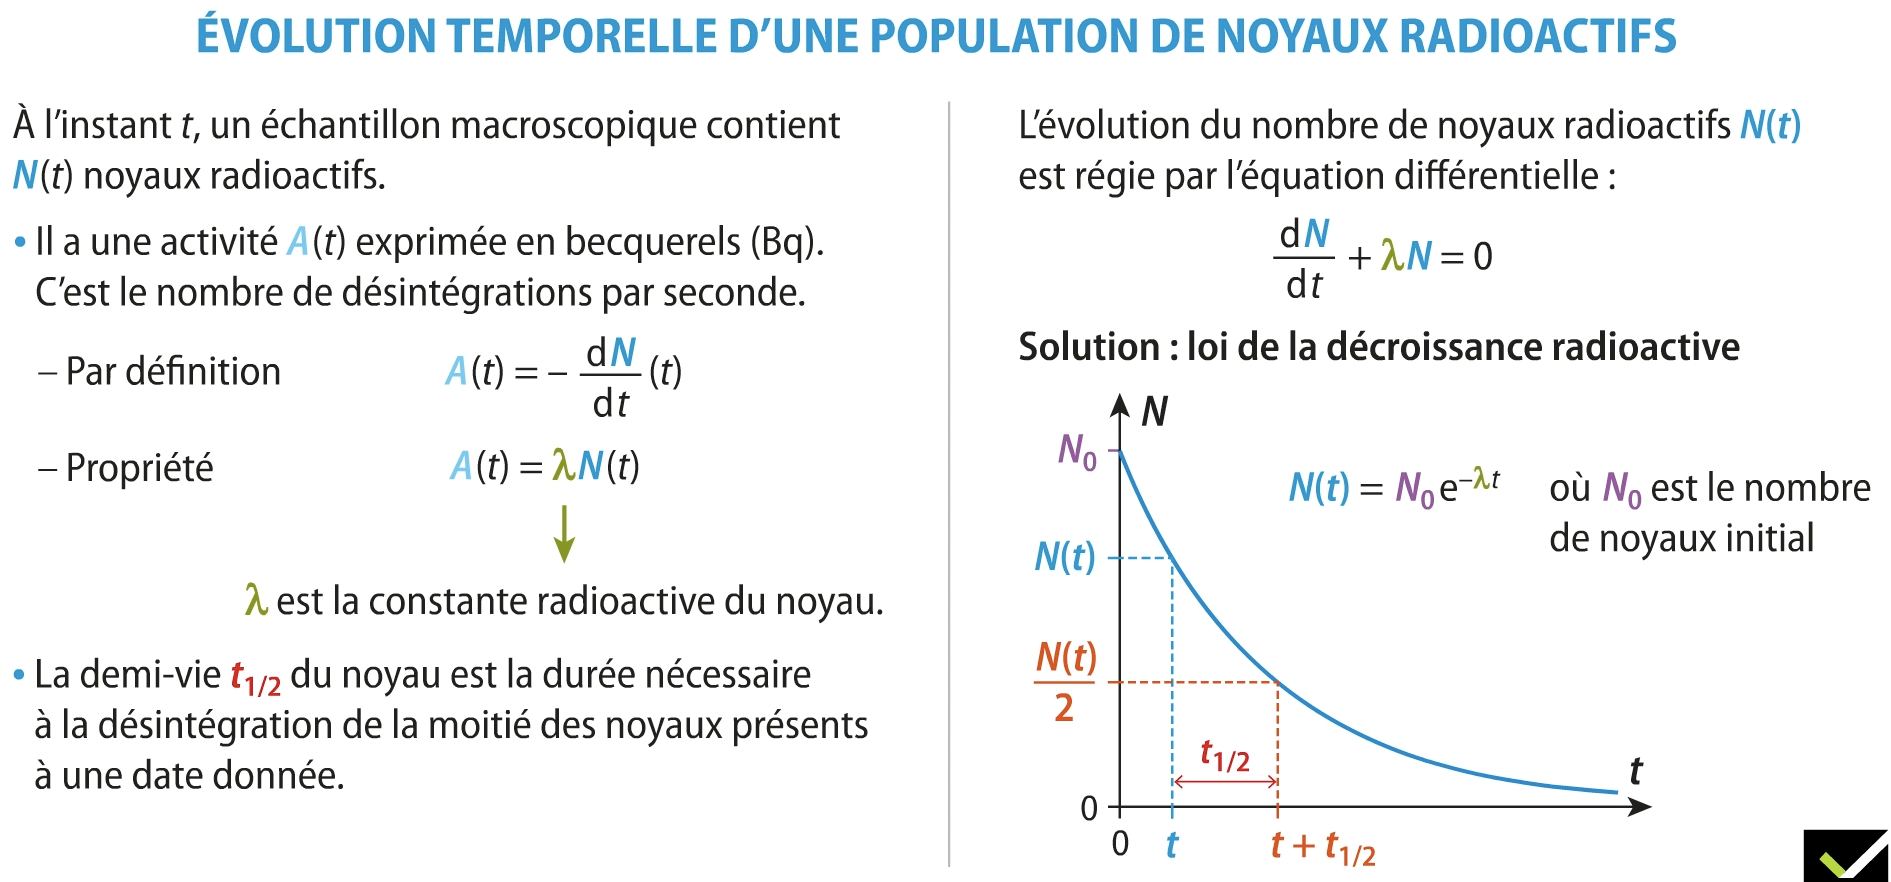
\includegraphics[width=.99\textwidth]{figures/nucleaire_resume.png}
\etiquetterouge{Exercices}

\begin{itemize}
	\item 6 , 12 p 122-123
	\item 19 p 124
	\item 27 et 32 p 126-128
\end{itemize}


